\subsection{Programming in ArBB}
\label{sec:ProgrammingArBB}

What the authors of ArBB call {\em latent parallelism} is expressed both
by using operations like scan and reduce (or fold) over vectors and by
mapping functions over collection data-types.
ArBB provides both dense and nested vectors. 
%The nested vectors permit 
%nested data parallelism (and are one of the attractions of ArBB).
% but we have not yet included them in our embedding. Thus, we consider only dense vectors here.
Dense vectors can be one, two or three dimensional; they correspond
to ordinary arrays.

%The vectors 
%in ArBB can be one, two or three dimensional dense vectors (in other words arrays)
%or nested vectors that allow the programmer to utilise nested data parallelism. 
%A nested vector is represented by an array of elements and an array holding a 
%nesting descriptor. 
% BJS: I have seen this elsewhere but cannot find it! (wanted to \cite something)
%The ArBB system offers the programmer {\em dense} and {\em nested} vectors 
%and operations on these. A dense vector (or simply put, an array) can 
%be one, two or three dimensional. A nested vector is represented by an 
%array of elements and an array holding a nesting descriptor. Nested vectors 
%can be used to express nested data-parallelism. 

Matrix-vector multiplication can be expressed in ArBB and C++ like this: 
\begin{Verbatim}[samepage=true] 
void arbb_matrix_vector(const dense<f32, 2>& a, 
                        const dense<f32>& x,
                        dense<f32>& b) {
  b = add_reduce(a * repeat_row(x, a.num_rows()));
}
\end{Verbatim} 
\noindent
This function takes a dense matrix (a two dimensional array), {\tt a}, and a dense vector, {\tt x},
and returns a dense vector {\tt b}.
It
uses {\tt add\_reduce} and {\tt repeat\_row}, which are built in ArBB 
operations. Note that we are not provided with a general reduction operator
that takes a function as parameter,
but rather with specific instances.
%The resulting code is automatically vectorised and threaded. 


The matrix-vector multiplication code above is very concise, but some further
steps are necessary before it can be run on real data. The code 
below shows how to set up a 4x4 scaling matrix and a vector to 
multiply by that matrix using ArBB. This entails allocating 
memory on the ArBB heap and copying data into it, reminiscent of the copying of
data from
host to 
device that is common in general purpose GPU (GPGPU) programming . 

%[samepage=true] 
\begin{Verbatim} 
int main(void)
{
  float matrix[4][4] = {{2.0,0.0,0.0,0.0},
                        {0.0,2.0,0.0,0.0},
                        {0.0,0.0,2.0,0.0},
                        {0.0,0.0,0.0,2.0}};
  float vector[4] = {1.0,2.0,3.0,4.0}; 

  // set up the matrix in ArBB 
  dense<f32, 2> a(4, 4);
  range<f32> write_a = a.write_only_range();
  float* a_ = &write_a[0];
  memcpy(a_,matrix,16*sizeof(float));

  // set up the vector in ArBB 
  dense<f32> x(4);
  range<f32> write_x = x.write_only_range();
  float* x_ = &write_x[0];
  memcpy(x_, vector,4*sizeof(float));

  // Room for the result
  dense<f32> arbb_b(4);
  const_range<f32> read_arbb_b;

  call(arbb_matrix_vector)(a, x, arbb_b);
  read_arbb_b = arbb_b.read_only_range();

  for (int i = 0; i < 4; ++i) {
    printf("%f ", read_arbb_b[i]);
  }
 
  return 0;
}
\end{Verbatim}

After setting up and copying the data into ArBB, the function {\tt arbb\_matrix\_vector} 
is {\em called} using the {\tt call} command. At this point, a number of
things happen. If the function is called for the first time, it is 
{\em captured}. This means that the function is run as a C++ function, which produces 
an intermediate representation (IR) of the computation (which is standard in such embeddings).
For example, if the function being captured contains a normal C++ {\em for loop}, it will be unrolled, much in the same way as recursion in a
Haskell embedded DSL results in unrolled code. After the function is captured, 
the IR is further optimised and finally executed. Compilation and capture 
only occur the first time a function is called. The compilation procedure
is outlined in~\cite{ARBB2011}.

Nested vectors in ArBB allow the creation of an array of dense vectors of varying length -- giving the ability to express less regular parallelism. There is a limit, though, in that only one level of such nesting is allowed. Section~\ref{sec:smvm} shows a small example that uses this nestedness in EmbArBB to implement sparse matrix vector multiplication. The program in ArBB itself is very similar. We note, though, that one of the samples distributed with ArBB is also sparse matrix vector multiplication, but implemented using dense vectors and a function that can take sections of a vector. We will need to experiment further with nestedness and when it should be used.

%In this document we describe early stages of work with a Haskell Embedding 
%of ArBB. We call this embedded language EmbArBB. It is our hope that using 
%Haskell as a host language will be just as user friendly and efficient as 
%the C++ version. Since this is work-in-progress there are places where 
%EmbArBB is lacking functionality that the C++ embedding has. This is the 
%case with nested vectors for example, more details in the Future Work section. 


%\FloatBarrier
\subsection{Programming in EmbArBB} 
\label{sec:Programming}


%** Note. The intro should mention that the current version of EmbArBB
%is available on github and say how to fetch it, I suppose.

In EmbArBB, ArBB functions are expressed as Haskell functions on expressions
(abstract syntax trees). This is standard Haskell embedded language procedure. 
A function that adds a constant to all elements of a vector is

\begin{verbatim}
addconst :: Num a 
          => Exp a 
          -> Exp (DVector Dim1 a) 
          -> Exp (DVector Dim1 a) 
addconst s v = v + ss 
    where 
      ss = constVector (length v) s 
\end{verbatim}

In this function {\tt (+)} is used for elementwise addition of two vectors. 
The function {\tt constVector} is part of the EmbArBB library and creates a vector 
of a given length containing the same value at each index. 

EmbArBB supports one, two and three dimensional dense vectors. These vectors are 
represented by a datatype called {\tt DVector} (for Dense Vector). {\tt DVector} takes two 
arguments, the first specifying its dimensionality and the second its payload 
type. Hence, an array of 32 bit words has type {\tt DVector Dim1 Word32}.
The one dimensional {\tt DVector} also has the alias {\tt Vector}. The type 
of the {\tt addconst} function above could also have been written: 

\begin{verbatim}
addconst :: Num a 
          => Exp a 
          -> Exp (Vector a) 
          -> Exp (Vector a) 
\end{verbatim}

The nested vectors of ArBB correspond to {\tt NVectors} in EmbArBB. 
%These vectors are called nested vectors in ArBB but are limited to one level of nesting.  

The {\tt addconst} function needs to be {\em captured} before it can be executed. 
The term {\em capture} is borrowed from ArBB nomenclature and corresponds to compiling 
the embedded language function into an ArBB function. In EmbArBB, a function is 
captured using the function {\tt capture}; in the C++ embedding, a function is 
captured when it is called for the first time. The same could have been done in 
the Haskell embedding of course, but we chose to make
capture explicit for simplicity.
The {\tt capture} function takes a Haskell function as input and produces an 
opaque typed function identifier as output. The identifier points out the function 
in an environment that is managed by a monad called {\tt ArBB}. To make this 
concrete, Figure~\ref{fig:EmbArBBcode1} shows the complete procedure from capturing 
to execution.  

%\begin{verbatim} 
%main = 
%  withArBB $ 
%  do 
%     f <- capture addconst
%     ...    
%\end{verbatim} 
 
The {\tt withArBB} function (line two) is the ``run''-function of the {\tt ArBB} monad. 
It turns something of type {\tt (ArBB a)} into {\tt (IO a)}. This is how ArBB 
computations are interfaced with Haskell. A {\tt withArBB} session also sets the scope 
for any captured functions or vectors created in the ArBB monad.

The result of {\tt capture addconst} on line four in the code has type 
%Function (Float :- Vector Float) 
%         (MDVector Dim1 Float)
\begin{verbatim}
Function (BEScalar Float :- BEDVector Dim1 Float) 
         (BEDVector Dim1 Float)
\end{verbatim}
representing a function that takes a float and a vector of floats as 
input and gives a vector of floats as result. The ``BE'' prefixes 
in those names ({\tt BEScalar},{\tt BEDvector}) refers to this being vectors and scalar that 
reside in the ArBB heap (Backend vectors). BEVectors and Scalars are mutable and the 
vector used to store the result needs to be allocated by the programmer. This interface 
seems rather imperative but ArBB requires output data to be
placed into an output vector of the correct size. 
Because of this, the options were either to try to infer result size (which can be dependent on the value of input data) or to have the programmer
supply storage for the result. We chose the latter, and thus also avoid
additional runtime overhead due to size inference.

%This means that the options where to either somehow 
%infer the result size automatically (if that is even feasible, output size 
%could potentially be data dependent) or to let the programmer supply storage 
%for the result. Inferring size would surely also impose extra runtime overhead. 

Continuing with the example: the function, once captured, can be executed 
on data. On line five, a {\tt DVector} is copied into ArBB using the {\tt copyIn} function. 
A vector to hold the result is created using the {\tt new} function on line eight. The 
{\tt new} function takes a shape description ({\tt (Z:.10)}, meaning a one dimensional 
vector of length 10) and an element to fill the vector with initially.
A scalar {\tt c} is created using {\tt mkScalar} on line nine. Next, on line ten, the 
function is executed by issuing 
\begin{verbatim}
execute f (c :- x) r1
\end{verbatim}
The {\tt (c :- x)} is a heterogeneous list of inputs. 
The {\tt :-} operator is similar to normal cons ({\tt :}) on Haskell lists.  
The output is stored in {\tt r1}. Had there been more outputs, the output
list would have also had a heterogeneous list type of the form
{\tt (r1 :- ... :- rn)}. If the result is a 
scalar, a storage location can be created using a function called 
{\tt mkScalar} that takes its initial value as input. 

All that remains is to copy the output vector out of ArBB and show the result; this 
is done on lines eleven and twelve in the figure.  

%main = 
% withArBB $ 
%  do 
%     f <- capture addconst
%     let x = fromList [0..10 :: Float]      
%     r1 <- liftIO$ new1D 10   
%     execute f (1 :- x)  r1   
%     r <- liftIO$ freeze r1             
%     liftIO$ putStrLn$ show r   
\begin{figure}
\begin{Verbatim}[numbers=left,frame=single] 
main = 
  withArBB $ 
  do 
     f <- capture addconst             
     x <- copyIn $ mkDVector 
                     (V.fromList [1..10 :: Float]) 
                     (Z:.10)
     r1 <- new (Z:.10) 0 
     c <- mkScalar 1      
     execute f (c :- x)  r1              
     r <- copyOut r1              
     liftIO$ putStrLn$ show r
\end{Verbatim}
\caption{The code shows how to capture a function, upload data to ArBB and 
         how to execute the captured function.}
\label{fig:EmbArBBcode1}
\end{figure}  
%$
%** Note, I think it would be best to put the code above into a figure and then just refer to it in the discussion, rather than have three versions of it of
%increasing size.

In this example, we have seen all of the important parts of the
Haskell to EmbArBB interface: how embedded language functions are compiled and
executed, and how to transfer data from Haskell into the ArBB world.
The following subsections show EmbArBB versions of some common 
data parallel computations.

% -- Get the number of columns
% getNCols :: Exp (DVector (t:.Int:.Int) a) 
%           -> Exp USize 



\begin{figure}
\begin{small}
\begin{Verbatim}
-- Scatter values into a vector 
-- resolves collisions by adding elements
addMerge :: Exp (DVector (t:.Int) USize) -- indices
         -> Exp USize                    -- res length
         -> Exp (DVector (t:.Int) a)     -- src
         -> Exp (DVector (t:.Int) a) 

-- Reduce a vector using addition
addReduce :: Num a 
          => Exp USize   -- rows, cols or pages
          -> Exp (DVector (t:.Int) a) 
          -> Exp (DVector t a) 

-- Segmented version of addReduce
addReduceSeg :: Num a 
             => Exp (NVector a)  -- nested input
             -> Exp (DVector Dim1 a)

-- Create a nested vector from a dense
applyNesting :: Exp USize  -- lengths or offsets
             -> Exp (DVector Dim1 USize) -- nesting
             -> Exp (DVector Dim1 a)     
             -> Exp (NVector a)


-- Create a vector with a constant value
constVector :: Exp USize  -- length
            -> Exp a      -- value
            -> Exp (DVector Dim1 a) 
\end{Verbatim}
\end{small}
\caption{A list of EmbArBB functions that are used in the examples with 
         short descriptions, part 1.} 
\label{fig:listoffunA}
\end{figure} 


\begin{figure}
\begin{small}
\begin{Verbatim}

-- Extract a column from a 2D vector
extractCol :: Exp USize              -- col. index
           -> Exp (DVector Dim2 a)  
           -> Exp (Vector a) 
 
-- Fill a portion of a vector with a constant 
fill :: Exp a                -- fill value 
     -> Exp USize            -- start 
     -> Exp USize            -- end 
     -> Exp (DVector Dim1 a) -- dst
     -> Exp (DVector Dim1 a) 

-- Gather elements from a vectors 
gather1D :: Exp (DVector Dim1 USize)  -- indices
         -> Exp a                     -- default
         -> Exp (DVector Dim1 a)      -- values
         -> Exp (DVector Dim1 a) 

-- Get the number of rows 
getNRows :: Exp (DVector (t:.Int:.Int) a) 
         -> Exp USize 

-- Turn a zero dimensional vector into a scalar 
index0 :: Exp (DVector Z a) -> Exp a 

-- Create a 2D vector by repeating a 1D vector
repeatRow :: Exp USize            -- #repetitions
          -> Exp (DVector Dim1 a) -- row
          -> Exp (DVector Dim2 a) 

-- Replace one column in a 2D vector 
replaceCol :: Exp USize            -- col
           -> Exp (DVector Dim1 a) -- new values
           -> Exp (DVector Dim2 a) 
           -> Exp (DVector Dim2 a) 

-- Convert every element of a vector to USize
vecToUSize :: Exp (Vector a) 
           -> Exp (Vector USize)

\end{Verbatim}
\end{small}
\caption{A list of EmbArBB functions that are used in the examples with 
         short descriptions, part 2.} 
\label{fig:listoffun}
\end{figure} 

\begin{figure}
\fbox{
\parbox{\linewidth}{
\begin{itemize}
\item {\tt ISize} is an integer type used to specify for example offsets.
\item {\tt USize} is an unsigned integer type used for lengths or indices.
\item {\tt Boolean} replaces the {\tt Bool} type for EmbArBB programs. The 
reason for this is that ArBB internally represents booleans as 8bit words.
while the {\tt Storable} instance for {\tt Bool} does not. 
\item {\tt DVector} is the type of regular shaped vectors.
\item {\tt NVector} is the type of irregularly shaped vectors.
\end{itemize}
}
}
\caption{A list of EmbArBB types with short descriptions} 
\label{fig:listoftyp}
\end{figure} 




In the examples one can assume that following imports have been made: 
\begin{verbatim}
import Data.Vector as V
import Prelude as P
\end{verbatim}
In this way, wherever there is potential for mixup between EmbArBB functions 
and Prelude or Data.Vector functions, these are prefixed by either ``{\tt V.}'' or 
``{\tt P.}''. 

% \FloatBarrier 
\subsubsection{Saxpy} 
{\em Saxpy} is a vector operation that gets its name from the 
description of what it does ``{\em S}ingle-precision {\em A}lpha {\em X} {\em P}lus {\em Y}''. 
There is also a double-precision version called {\em daxpy}. Here we can use a single source 
to obtain both versions:
%. The code listing below {\em axpy} illustrates this: 

\begin{verbatim} 
saxpy :: Num a 
      => Exp a 
      -> Exp (DVector Dim1 a) 
      -> Exp (DVector Dim1 a) 
      -> Exp (DVector Dim1 a) 
saxpy s x y = (ss*x) + y 
    where 
      ss = constVector (length x) s
\end{verbatim}

Now, {\tt capture} can be used to instantiate the function at either float or double 
types.  

\begin{verbatim}
main = 
  withArBB $ 
  do 
     f <- capture saxpy
     
     let v1 = V.fromList [1,3..10::Float] 
         v2 = V.fromList [2,4..10::Float] 
          
     x <- copyIn $ mkDVector v1 (Z:.5) 
     y <- copyIn $ mkDVector v2 (Z:.5) 
     
     r1 <- new (Z:.5) 0    
           
     c <- mkScalar 1 
     
     execute f (c :- x :- y)  r1
              
     r <- copyOut r1
              
     liftIO$ putStrLn$ show r
\end{verbatim}

%If instead the double precision version was desired change just the 
%type at which the function is captured. In the example above this 
%amounts to changing {\tt ::Float} to {\tt ::Double} in the definitions 
%of {\tt v1} and {\tt v2}. 

Changing {\tt Float} to {\tt Double} in the definitions 
of {\tt v1} and {\tt v2} gives the double precision version of the function.
%Here, the two different choices for the type of the data lead to
%two different generated ArBB functions. 
A function needs to be captured at every type at which it is to be used. This 
is because the resulting ArBB function is not polymorphic over something corresponding 
to {\tt Num} types (while the embedded language function is). 

\subsubsection{Matrix-vector multiplication} 
In section~\ref{sec:ProgrammingArBB}, matrix-vector multiplication was shown using the C++ ArBB interface. 
Here, EmbArBB is used to implement the same function. The function definition itself 
is very similar to the C++ one:

\begin{verbatim} 
matVec :: Exp (DVector Dim2 Float) 
        -> Exp (DVector Dim1 Float) 
        -> Exp (DVector Dim1 Float) 
matVec m v = addReduce rows 
           $ m * (repeatRow (getNRows m) v)

\end{verbatim} 

The {\tt addReduce} function takes a parameter that specifies whether to reduce 
rows or columns. 

% ** Note. What is a level specifier?

The following Haskell {\tt main} function completes the comparison to the C++ version shown in the Introduction:

\begin{verbatim}
main =  
  withArBB $ 
  do 
     f <- capture matVec  
     let m1 = V.fromList [2,0,0,0,
                          0,2,0,0,
                          0,0,2,0,
                          0,0,0,2]
         v1 = V.fromList [1,2,3,4] 
     
     m <- copyIn $ mkDVector m1 (Z:.4:.4) 
     v <- copyIn $ mkDVector v1 (Z:.4) 

     r1 <- new (Z:.4) 0 

     execute f (m :- v)  r1
              
     r <- copyOut r1
              
     liftIO$ putStrLn$ show r
\end{verbatim}
%$ -- fixes syntax highlighting
The complete Haskell version of this program is slightly shorter than the corresponding 
C++ version. However, the C++ version could probably be made shorter as well; the Haskell and C++ versions must be considered similar in implementation complexity. 

%This is 
%a very short example and cannot be expected to show off the strengths of either language. 

\subsubsection{Matrix-matrix multiplication}

%Matrix multiplication is studied in the benchmarks in section~\ref{sec:Benchmarks}.
The following EmbArBB implementation of matrix-matrix multiplication is used as a benchmark in section~\ref{sec:EmbArBBBenchmarks}:

\begin{verbatim} 
matmul :: Exp (DVector Dim2 Float) 
        -> Exp (DVector Dim2 Float) 
        -> Exp (DVector Dim2 Float) 
matmul a b = fst $ while cond body (a,0)
  where 
    m = getNRows a
    n = getNCols b 
    cond (c,i) = i <* n
    body (c,i) = 
      let mult = a * repeatRow m (extractCol i b)
          col  = addReduce rows mult 
      in (replaceCol i col c, i+1) 
\end{verbatim}

This example uses a {\tt while} loop. In the C++ embedding of ArBB, the programmer 
has the option of using a C++ {\tt while} loop or a special {\tt while\_} loop. The 
normal C++ while loop unrolls at capture time; the {\tt while\_} is kept by ArBB 
and corresponds to an ArBB loop. The two loops differ in the kinds of
values on which they can depend.
The C++ loop can only depend on C++ values, so
the number of iterations in a normal {\tt while} loop must be known at capture 
time. All of these concepts have Haskell counterparts. The {\tt while} loop used in the 
example corresponds to the {\tt while\_} loop and will remain in the generated ArBB 
code; it can depend on ArBB values at runtime.
Haskell recursion is used to get the kind of unrolling 
that one gets by using a C++ {\tt while} loop. 
 
The EmbArBB {\tt while} loop takes three parameters, a condition, a body and an initial state. 
In every iteration of the loop, the body is applied to the state and the condition checked.

%Using {\tt a}, that is the input matrix, as initial state may seem strange but it relies 
%on that the implementation of the while loop creates a copy of the initial state that 
%is used in the iterations. This makes the {\tt while} loop slightly unclear in what it 
%does and is something that must be improved as future work. An improvement could be 
%if the programmer specified {\tt (newMatrix m n,0)} as initial state. 

\subsubsection{Histogram}
\FloatBarrier

The histogram of a grayscale image contains the frequency with 
which each shade occurs in the image. In this example, the image used represents 
the shade of each pixel with a single byte, so that
256 different shades are possible. An array of length 256 is created to hold at index 
{\tt i} the number of occurrences of the shade {\tt i} in the image. In essence, this 
is an array of buckets. 

\begin{verbatim}
histogram :: Exp (DVector Dim2 Word8)  
           -> Exp (Vector Word32)
histogram input = addMerge (vecToUSize flat) 256 cv
    where
      flat = flatten input
      cv = constVector (r * c) 1 
      r  = getNRows input 
      c  = getNCols input
      
\end{verbatim}

The {\tt addMerge} operation takes a vector of inputs, a vector of 
indices and finally a size (specifying the result size). Elements from the 
input vector ({\tt cv} in the example) are placed into the result
at the index specified at 
the same location in the indices vector. Elements placed at the same
index are added together. Here, the input vector contains all ones, 
while the image is {\em cast} into a vector of indices.
The result 
is that index {\tt i} of the output vector contains the number of times
shade {\tt i} appears in the image.
The histogram
computation becomes very concise through the use of the {\tt addMerge} operation.

The code below creates the image shown in figure~\ref{fig:histogram}. It 
takes as input a vector on frequencies and outputs a two dimensional vector, 
a grayscale image. 

\begin{verbatim}
histImage :: Exp (Vector Word32) 
           -> Exp (DVector Dim2 Word8) 
histImage input = fst $ while cond body (cvn,0)    
    where 
      cond (img,i) = i <* n 
      body (img,i) = (replaceCol i col' img,i+1) 
          where 
            val = input ! i 
            col = extractCol i img
            col' = fill black 0 n col
            n = 255 - scale 255 m val  
                    
      n = length input 
      cv = constVector (n*n) white  
      cvn = setRegularNesting2D n n cv
      m   = index0 (maxReduce rows input)
      black = 0 
      white = 255
\end{verbatim}

\begin{figure} 
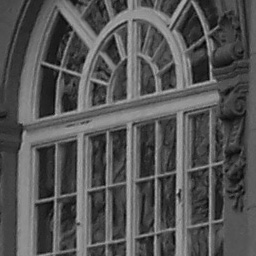
\includegraphics[width=.5\linewidth]{./embarbb/img/window}
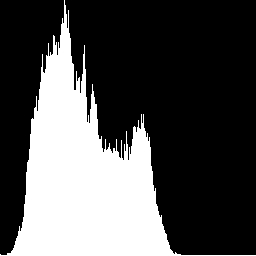
\includegraphics[width=.5\linewidth]{./embarbb/img/histogram}
\caption{ The righ-hand image visualises the frequency with which 
          different shades of gray occur in the left-hand one.}
\label{fig:histogram}
\end{figure} 

\FloatBarrier
\subsubsection{Sobel edge detection filter}
\label{sec:Sobel}
\FloatBarrier 

Sobel edge detection is an example of a stencil computation
over an array. At each element of the array, a computation is 
performed that depends on that element and on elements close by. Which of the nearby 
elements to use, and how much they influence the result is typically described using a matrix 
(in the two dimensional case) called the stencil. Below are two stencils used in the 
sobel edge detection filter: 

\begin{minipage}{0.5\linewidth}
\[
G_x = \begin{bmatrix*}[r]
        -1 & 0 & 1 \\ 
        -2 & 0 & 2 \\
        -1 & 0 & 1 
      \end{bmatrix*}
\]
\end{minipage}
\begin{minipage}{0.5\linewidth}\centering
\[
G_y = \begin{bmatrix*}[r]
        -1 & -2 & -1 \\ 
         0 &  0 &  0 \\
         1 &  2 &  1 
      \end{bmatrix*}
\]
\end{minipage}

In ArBB, the {\em map} operation gives the programmer a way to implement stencil computation. 
It takes a function and a vector on which to apply the function at each element. 
Inside the function being mapped, the programmer may use a set of {\em getNeighbor} functions 
to access nearby elements. 

The elements used by the stencils are kept (in the form of
coordinates relative to the centre point of the matrix) in two Haskell lists. This is an 
example of how host language (Haskell) features are used as a kind of 
scripting aid. 

\begin{verbatim} 
s1, s2 :: [(Exp ISize,Exp ISize)]
s1 = [(1,1),(0,1),(-1,1),(1,-1),(0,-1),(-1,-1)]
s2 = [(1,1),(1,0),(1,-1),(-1,1),(-1,0),(-1,-1)]
\end{verbatim} 

The actual weights are placed in a separate list. 

\begin{verbatim} 
coeffs :: [Exp Float] 
coeffs = [-1,-2,-1,1,2,1] 
\end{verbatim}

The following functions implement the stencil computation part of the program
using the elements pointed out by {\tt s1} and {\tt s2} together with  the weights in {\tt coeffs}. 
Each of the six neighbours is multiplied by the appropriate weight. 
Haskell's {\tt foldl} function is used to sum up the values, to
give the result for the location in question. Using a Haskell fold means that the 
summation is unrolled. 

\begin{verbatim}
gx :: Exp Word8 -> Exp Float  
gx x = P.foldl (+) 0 
     $ P.zipWith (*) [toFloat (getNeighbor2D x a b) 
                      / 255 
                     | (a,b) <- s1] coeffs 


gy :: Exp Word8 -> Exp Float 
gy x = P.foldl (+) 0 
     $ P.zipWith (*) [toFloat (getNeighbor2D x a b) 
                      / 255
                     | (a,b) <- s2] coeffs 
\end{verbatim}

The helper functions {\tt convertToWord8} and {\tt clamp} take 
care of converting floats between 0 and 1 to bytes between 0 and 255, and 
of clamping floating point values into the 0 to 1 range. 

\begin{verbatim}
convertToWord8 :: Exp Float -> Exp Word8 
convertToWord8 x = toWord8 $ (clamp x)  * 255

clamp :: Exp Float -> Exp Float
clamp x = max 0 (min x 1)  
\end{verbatim}

The complete kernel, the program that is to be executed at every index of the image,
is given below. The earlier parts are brought together into a function that 
transforms one {\tt Word8} into another. 

\begin{verbatim} 
kernel :: Exp Word8 -> Exp Word8 
kernel x = convertToWord8 $ body x
  where 
    body x = sqrt (x' * x' + y' * y') 
     where 
       x' = gx x 
       y' = gy x
\end{verbatim}
\noindent
In order to execute the kernel, an ArBB {\tt map} is used. 
%ArBB map allows the function being 
%mapped to access elements neighbouring the current index by the {\tt getNeighbor} 
%functions. 

\begin{verbatim}
sobel :: Exp (DVector Dim2 Word8) 
         -> Exp (DVector Dim2 Word8) 
sobel image = map kernel image  
\end{verbatim} 

%In the current version of EmbArBB, the {\tt sobel} function needs to take as input 
%the function that it passes to map. This gives the {\tt sobel} function the somewhat
%complicated type that it has above. The reason the function needs to be passed as input 
%is that the {\tt kern} used in {\tt map kern image} is an opaque {\tt Function} object, 
%that is a result of calling {\tt capture}. Capturing is an operation in the {\tt ArBB} 
%monad and it is in that monad that the actual map of opaque {\tt Function} objects to 
%already generated ArBB functions is kept. 
%We see this as a wart on the current implementation.
%In future work, we would like to simplify matters for the user. 

The implementation of {\tt sobel} is pleasingly simple and concise in this setting. 
Despite the fact that this is a small example, the value of being able to use Haskell
lists and operations is already becoming obvious.
%Making 
%use of Haskell lists and operations as powerful scripting tools. 

\begin{figure}
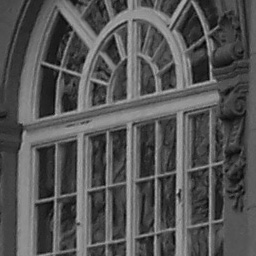
\includegraphics[width=.5\linewidth]{./embarbb/img/window}
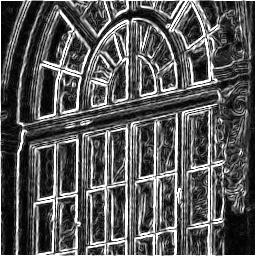
\includegraphics[width=.5\linewidth]{./embarbb/img/sobout}
\caption{ The image on the right shows the result of applying the sobel edge 
          detection filter to that on the left. }
\label{fig:sobel}
\end{figure}


%\subsection{Functions, Capturing and Executing}

%\subsection{Moving data to and from ArBB}

%\subsection{Programming Examples}
\FloatBarrier

\subsubsection{Image filtering} 
\label{sec:Blur}
The blur operation, which is a kind of spatial linear filter, shows another way to implement a stencil operation. The {\tt mapStencil} function used is a composite 
function in the EmbArBB library; it is not provided as a primitive from 
the ArBB VM. 

\begin{verbatim} 
blur :: Exp (DVector Dim2 Word8) 
        -> Exp (DVector Dim2 Word8) 
blur image = vec2DToWord8 (res `div`  all16) 
  where 
    all16 = constVector2D (getNRows image) 
                          (getNCols image)
                          16
    res = mapStencil (Stencil [1,2,1
                              ,2,4,2   
                              ,1,2,1] (Z:.3:.3)) 
                     image' 
     
    image' = vec2DToWord32 image        
\end{verbatim}

In Repa, similar {\tt mapStencil} functionality is present but using Template 
Haskell to give a safer way to specify the stencil. In our version there is 
no protection agains mischievous stencil specification. This guarantees only
that if the programmer says the stencil is two dimensional then it can only 
be applied to two dimensional vectors. Applying similar Template Haskell based
extension here as well is probably quite easy now that Repa has shown how.

\subsubsection{Sparse matrix multiplication}\label{sec:smvm}
A sparse matrix can be represented by three vectors, one (cidx) containing
column indices, one (offsets) indicating indices in the vector of values
at which the first non-zero element of each row appears, and one containing the
values themselves. This is known as the Compressed Sparse Row (CSR) format.
Given such a matrix and a dense vector, the relevant elements of the dense vector
can be gathered into a new vector using the column indices. The resuting vector
is multiplied pointwise by the vector of non-zero values from the sparse matrix. All that remains, then, is to divide the result into rows and sum each one. The offsets vector
points to where the division should happen.
The code in EmbArBB is as follows:

\begin{verbatim} 
smvm :: Exp (Vector USize)
     -> Exp (Vector USize)
     -> Exp (Vector Float)
     -> Exp (Vector Float)
smvm mval cidx os vec = addReduceSeg nps 
    where 
      ps = mval * gather1D cidx 0 vec
      nps = applyNesting offsets os ps 
\end{verbatim} 

The multiplication acts pointwise on the elements of {\tt vals}
and the vector (of the same length) containing relevant elements of the dense vector (produced using {\tt gather1D}).
The function {\tt applyNesting} produces
a nested vector of rows. The function {\tt addReduceSeg} sums each
of the rows (or segments) in that array, producing the non-zero elements
of the result vector. Note that there is irregular data parallelism
here because the rows may have different lengths. We would hope
to get parallelism both in the individual summations and between summations.
This is a well known algorithm that can be traced back to Blelloch~\cite{NESL}.

%% NOTE ** I took out the 0 in the parameters to gather1D. How about
%% we just assume it is forward for now (and put in the zero in the call
%% to Gather)

%\begin{verbatim}
%import Data.Vector.Storable as V 

%data DVector d a = Vector (V.Vector a) Dim 

%data Dim = Zero 
%         | One Int
%         | Two Int Int 
%         | Three Int Int Int 
%\end{verbatim} 

